\documentclass{article}
%\RequirePackage[T1]{fontenc}
\usepackage[screen]{tuepdfscreen}
\usepackage{graphicx, fleqn, tabularx, wrapfig}
\usepackage[ansinew]{inputenc}
\usepackage[spanish]{babel}
\usepackage{pifont}
\usepackage{times}
\usepackage{zahlen}%
%\setcounter{MaxMatrixCols}{30}%
\usepackage{amsfonts}%
\usepackage{amssymb}
\hypersetup{
  pdfauthor={Antalcides Olivo},
  pdftitle={INDUCCI�N AL LABORATORIO },
  pdfsubject={pdfscreen},
  pdfkeywords={pdfscreen,hyperref,presentaties,presentations,slides,latex,miktex},
  pdfpagemode={FullScreen}
}

%%
%% Navigation buttons at the bottom
%%
\bottombuttons
%%
%% Page numbers at the bottom
%%
\pagenumbering
%%
%% Background image
%%
\overlay{pdfslide.png}

\title{\Huge F�sica Calor Ondas\\\Large Laboratorio}
\author{\Large Universidad Del Norte}
\date{\large 12 de agosto del 2003}
\begin{document}

\newenvironment{descrsf}[1]
  {\begin{list}{}{\renewcommand{\makelabel}[1]{\textsf{##1}\hfil}
                  \setlength{\itemsep}{0.5em}
                  \setlength{\parsep}{0pt}
                  \settowidth{\labelwidth}{\textsf{#1}}
                  \setlength{\labelsep}{10pt}
                  \setlength{\leftmargin}{\labelwidth}
                  \addtolength{\leftmargin}{\labelsep}
                 }
  }
  {\end{list}}

\renewcommand{\descriptionlabel}[1]%
   {\hspace{\labelsep}\textsf{#1}}

\begin{slide}
\maketitle
\end{slide}
\begin{slide} \setlength{\parskip}{0.5cm}
{\textbf{\large{
\section{Introduction}
\textcolor[rgb]{0.00,0.00,0} {La idea de esta inducci�n es recordar
como utilizar el software Data Studio como herramienta para
interpretar fen�menos f�sicos y obtener resultados acorde con la
teor�a dada en clase, adem�s explicaremos como realizar ajuste de
datos a curvas y realizar c�lculos de error e interpretarlos}}}}
\end{slide}
\begin{slide}
\section{Normas}
\begin{enumerate}

    \item No consumir alimentos dentro del laboratorio
    \item No usar celulares ni otros tipos de aparatos de comunicaci�n
    \item No utilizar otro programa que no sea Data studio o la impresora.
    \item No manipular los equipos hasta que el profesor no de las instrucciones de seguridad
    \item No debe colocar �tiles u objetos en la mesa de trabajo, col�quelos en el entrepa�o de la mesa
    \item no debe llegar
\end{enumerate}
\end{slide}
\begin{slide}
\section{AN\'{A}LISIS GR\'{A}FICO}
El \ an\'{a}lisis gr\'{a}fico es un m\'{e}todo que nos sirve para determinar
la relaci\'{o}n matem\'{a}tica entre dos o m\'{a}s variables, ( en nuestro
caso cantidades f\'{\i}sicas) partiendo de una gr\'{a}fica realizada a partir
de datos experimentales tomados al azar.
Este estudio lo vamos presentar en tres partes :\newline Presentaci\'{o}n de
la gr\'{a}fica, escogencia de un modelo matem\'{a}tico y establecimiento de la
relaci\'{o}n emp\'{\i}rica entre las variables, pero antes explicaremos como
se introducen los datos en el software llamado Data Studio, el cual
utilizaremos en todo el semestre
\begin{enumerate}
\item Usando el sensor.
 El sensor transforma su lectura en datos
num\'{e}ricos usando la interface como puente entre el sensor y el software,
lo que quiere decir que los datos son introducidos automaticamente, y si hace
click en el icono table observara algo parecido a la Figura 1
%TCIMACRO{\FRAME{dhFU}{1.1381in}{1.8922in}{0pt}{\Qcb{Figura 1}}{\Qlb{figura1}%
%}{table.jpg}{\special{ language "Scientific Word";  type "GRAPHIC";
%maintain-aspect-ratio TRUE;  display "USEDEF";  valid_file "F";
%width 1.1381in;  height 1.8922in;  depth 0pt;  original-width 1.1044in;
%original-height 1.8542in;  cropleft "0";  croptop "1";  cropright "1";
%cropbottom "0";  filename 'table.jpg';file-properties "XNPEU";}}}%
%BeginExpansion
\centering
\includegraphics[
width=1.1381in]%
{table.png}\\%
Figura 1
%
%%EndExpansion
\item Editando una tabla.
 En la barra de men\'{u} est\'{a}ndar
se\~{n}ale experiment y haga click en new empty data table Figura 2%
%TCIMACRO{\FRAME{dhFU}{1.4313in}{1.6613in}{0pt}{\Qcb{Nueva tabla}%
%}{\Qlb{figura2}}{table2.jpg}{\special{ language "Scientific Word";
%type "GRAPHIC";  maintain-aspect-ratio TRUE;  display "USEDEF";
%valid_file "F";  width 1.4313in;  height 1.6613in;  depth 0pt;
%original-width 1.3958in;  original-height 1.625in;  cropleft "0";
%croptop "1";  cropright "1";  cropbottom "0";
%filename 'table2.jpg';file-properties "XNPEU";}}}%
%BeginExpansion
\centering
\includegraphics[
width=1.4313in]%
{table2.jpg}%
\\
Nueva tabla
\label{Figura 2}%
%EndExpansion
luego aparece una tabla como la de Figura 2.
%TCIMACRO{\FRAME{dhF}{2.7025in}{2.0332in}{0pt}{}{\Qlb{Figura2}}{datos1.jpg}%
%{\special{ language "Scientific Word";  type "GRAPHIC";
%maintain-aspect-ratio TRUE;  display "USEDEF";  valid_file "F";
%width 2.7025in;  height 2.0332in;  depth 0pt;  original-width 8.3333in;
%original-height 6.25in;  cropleft "0";  croptop "1";  cropright "1";
%cropbottom "0";  filename 'datos1.jpg';file-properties "XNPEU";}}}%
%BeginExpansion
\centering
\includegraphics[
width=2.7025in]%
{datos1.jpg}%
Figura 2%
%EndExpansion
Usando tab puede cambiar de celda para introducir datos.
\end{enumerate}
En caso de que se equivoque se puede borrar, se\~{n}alando y haciendo click
con el boton derecho en remove
\subsection{Presentaci\'{o}n de la gr\'{a}fica}
De acuerdo con el nivel de estas notas s\'{o}lo presentaremos una
introducci\'{o}n del an\'{a}lisis gr\'{a}fico en dos variables. las cuales
representaremos en un plano cartesiano de la siguiente forma:
\begin{enumerate}
\item Titulo:
El titulo lo colocamos en la parte superior as\'{\i}
(nombre de la variable en el eje $Y$) VS (nombre de la variable en el
eje $X$).
\item En los ejes las letras que representan a las variables y a sus unidades.
Se indican las escalas las cuales deben ser m\'{u}ltiplos de 2, 5 o 10
\item Luego se grafican los puntos siguiendo algunos de los siguientes m\'{e}todos
\begin{enumerate}
\item Se grafican los puntos y luego se intercala la gr\'{a}fica entre los
puntos, teniendo en cuenta que la gr\'{a}fica sea suave ( es decir que no
tenga v\'{e}rtices) y que la misma cantidad de puntos quede a un lado que al
otro de la gr\'{a}fica. por ejemplo%
%TCIMACRO{\FRAME{dtbpFU}{8.8194cm}{3.5981cm}{0pt}{\Qcb{Figura 1}}{\Qlb{Figura
%1}}{ajuste1.wmf}{\special{ language "Scientific Word";  type "GRAPHIC";
%maintain-aspect-ratio TRUE;  display "PICT";  valid_file "F";
%width 8.8194cm;  height 3.5981cm;  depth 0pt;  original-width 5.4864in;
%original-height 2.028in;  cropleft "0";  croptop "1";  cropright "1";
%cropbottom "0";  filename 'D:/Tacho/ajuste1.WMF';file-properties "XNPEU";}}}%
%BeginExpansion
\centering
\includegraphics[
width=8.8194cm]%
{ajuste1.jpg}%
\\
Figura 1
%EndExpansion
No se deba trazar as\'{\i}:%
%TCIMACRO{\FRAME{dtbpFU}{11.1237cm}{4.4372cm}{0pt}{\Qcb{Figura 2}}{\Qlb{Figura
%2}}{ajuste2.wmf}{\special{ language "Scientific Word";  type "GRAPHIC";
%maintain-aspect-ratio TRUE;  display "PICT";  valid_file "F";
%width 11.1237cm;  height 4.4372cm;  depth 0pt;  original-width 5.4864in;
%original-height 2.1664in;  cropleft "0";  croptop "1";  cropright "0.9998";
%cropbottom "0";  filename 'D:/Tacho/ajuste2.WMF';file-properties "XNPEU";}}}%
%BeginExpansion
\centering
\includegraphics[
height=4.4372cm,
width=11.1237cm
]%
{ajuste2.jpg}%
\\
Figura 2
%
%EndExpansion
En las figura 1 observamos que se pueden trazar infinitas gr\'{a}ficas que
cumplen las condiciones establecidas. \newline Lo que nos indica que la
gr\'{a}fica que trazamos no es la gr\'{a}fica real, \'{e}sta s\'{o}lo nos
indica su forma.
\item Si al tomar los datos podemos fijar cada medida de una variable Por
ejemplo: fijamos cada medida $x_{i}$ de $X$ entonces realizamos varios ensayos
para determinar cada valor $y_{i}$ de la variable $Y$, obteniendo la media
$\bar{y}_{i}$ para cada medida, luego graficamos para cada medida los puntos
$\left(  x_{i},\bar{y}_{i}\right)  ,\left(  x_{i},y_{M\acute{a}x}\right)  $ y
$\left(  x_{i},y_{m\acute{\imath}n}\right)  $ como indica la figura
%TCIMACRO{\FRAME{dtbpFU}{2.0245in}{2.0107in}{0pt}{\Qcb{Figura 3}}{}%
%{ydes.wmf}{\special{ language "Scientific Word";  type "GRAPHIC";
%maintain-aspect-ratio TRUE;  display "PICT";  valid_file "F";
%width 2.0245in;  height 2.0107in;  depth 0pt;  original-width 1.9865in;
%original-height 1.9726in;  cropleft "0";  croptop "1";  cropright "1";
%cropbottom "0";  filename 'D:/Tacho/ydes.WMF';file-properties "XNPEU";}}}%
%BeginExpansion
\centering
\includegraphics[
height=2.0107in,
width=2.0245in
]%
{ydes.jpg}%
%EndExpansion
Luego con una serie de datos trazamos una gr\'{a}fica que pase por la
mayor\'{\i}a de los puntos medios o que toque todos los segmentos, as\'{\i}:%
%TCIMACRO{\FRAME{dtbpFU}{1.8922in}{1.8334in}{0pt}{\Qcb{Figura 4}}{}%
%{gdes.wmf}{\special{ language "Scientific Word";  type "GRAPHIC";
%maintain-aspect-ratio TRUE;  display "PICT";  valid_file "F";
%width 1.8922in;  height 1.8334in;  depth 0pt;  original-width 2.6247in;
%original-height 2.5417in;  cropleft "0";  croptop "1";  cropright "1";
%cropbottom "0";  filename 'D:/Tacho/gdes.WMF';file-properties "XNPEU";}}}%
%BeginExpansion
\centering
\includegraphics[
height=1.8334in,
width=1.8922in
]%
{gdes.jpg}%
%EndExpansion
observemos que los segmentos indican la variabilidad de cada medida, es decir
la medida real puede ser cualquier valor sobre el segmento, lo que nos indica
que la curva real es una de las infinitas que podemos trazar entre las
gr\'{a}ficas punteadas, lo que indica que este m\'{e}todo me determina la
forma de la curva real.
\item Si cada medida $\left(  x_{i},y_{i}\right)  $ la obtenemos al realizar
varios ensayos, entonces graficamos cada punto $\left(  \bar{x}_{i},\bar
{y}_{i}\right)  $ tal que este en la intersecci\'{o}n de las diagonales del
rect\'{a}ngulo formado por los lados de longitudes $\Delta x_{i},\Delta y_{i}$
como indica la figura 5%
%TCIMACRO{\FRAME{dtbpFU}{2.0833in}{1.5696in}{0pt}{\Qcb{Figura 5}}{}%
%{destg.wmf}{\special{ language "Scientific Word";  type "GRAPHIC";
%maintain-aspect-ratio TRUE;  display "PICT";  valid_file "F";
%width 2.0833in;  height 1.5696in;  depth 0pt;  original-width 2.0557in;
%original-height 1.542in;  cropleft "0";  croptop "1";  cropright "1";
%cropbottom "0";  filename 'D:/Tacho/destg.WMF';file-properties "XNPEU";}}}%
%BeginExpansion
\centering
\includegraphics[
height=1.5696in,
width=2.0833in
]%
{destg.jpg}%
%EndExpansion
Con una serie de datos la curva debe pasar por todos los rect\'{a}ngulos como
indica la figura 6.%
%TCIMACRO{\FRAME{dphFU}{6.6031cm}{6.379cm}{0pt}{\Qcb{Figura 6}}{}%
%{gdes1.wmf}{\special{ language "Scientific Word";  type "GRAPHIC";
%maintain-aspect-ratio TRUE;  display "PICT";  valid_file "F";
%width 6.6031cm;  height 6.379cm;  depth 0pt;  original-width 6.4307in;
%original-height 6.2085in;  cropleft "0";  croptop "1";  cropright "1";
%cropbottom "0";  filename 'D:/Tacho/gdes1.WMF';file-properties "XNPEU";}}}%
%BeginExpansion
\centering
\includegraphics[
width=6.379cm
]%
{gdes1.jpg}%
%EndExpansion
De la figura observamos lo mismo que en los dos m\'{e}todos anteriores, que la
gr\'{a}fica que podemos trazar no es \'{u}nica
\end{enumerate}
\item Si usamos Data Studio, se hace lo siguiente.
\begin{enumerate}
\item Cuando digit\'{o} los datos observe que en la parte superior derecha de
la ventana aparecieron los siguientes iconos Figura 3,,
%TCIMACRO{\FRAME{dhF}{2.5728in}{1.8706in}{0pt}{}{\Qlb{figura3}}{datas.jpg}%
%{\special{ language "Scientific Word";  type "GRAPHIC";
%maintain-aspect-ratio TRUE;  display "USEDEF";  valid_file "F";
%width 2.5728in;  height 1.8706in;  depth 0pt;  original-width 2.5313in;
%original-height 1.8334in;  cropleft "0";  croptop "1";  cropright "1";
%cropbottom "0";  filename 'datas.jpg';file-properties "XNPEU";}}}%
%BeginExpansion
\centering
\includegraphics[
width=2.5728in
]%
{datas.jpg}%
%
%EndExpansion
haga clic sobre el l\'{a}piz, para que aparezca%
%TCIMACRO{\FRAME{dhF}{2.7025in}{2.0332in}{0pt}{}{}{editable.jpg}%
%{\special{ language "Scientific Word";  type "GRAPHIC";
%maintain-aspect-ratio TRUE;  display "USEDEF";  valid_file "F";
%width 2.7025in;  height 2.0332in;  depth 0pt;  original-width 8.3333in;
%original-height 6.25in;  cropleft "0";  croptop "1";  cropright "1";
%cropbottom "0";  filename 'editable.jpg';file-properties "XNPEU";}}}%
%BeginExpansion
\centering
\includegraphics[
width=2.7025in
]%
{editable.jpg}%
%
%EndExpansion
\item prueba
aaaa
\begin{descrsf}{xlabel}
\item Haciendo click en xlabel, ylabel puede colocar en label el nombre de las
variables,(en \'{\i}ngles si trabaja con sensores y el programa no est\'{a}
traducido), en units coloca las unidades corespondientes a la variable en el
sistema internacional (SI)
\item El t\'{\i}tulo se coloca en measurement, en accuracy se coloca la
precisi\'{o}n y en display precision el n\'{u}mero de cifras decimales
\item Haciendo click sobre el tri\'{a}ngulo o figura que aparece debajo del
l\'{a}piz y se arrastra hasta graph como indica la figura4
%TCIMACRO{\FRAME{dhF}{0.7187in}{1.0862in}{0pt}{}{\Qlb{figura4}}{graph.jpg}%
%{\special{ language "Scientific Word";  type "GRAPHIC";
%maintain-aspect-ratio TRUE;  display "USEDEF";  valid_file "F";
%width 0.7187in;  height 1.0862in;  depth 0pt;  original-width 0.6875in;
%original-height 1.0525in;  cropleft "0";  croptop "1";  cropright "1";
%cropbottom "0";  filename 'graph.jpg';file-properties "XNPEU";}}}%
%BeginExpansion
\centering
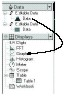
\includegraphics[
width=0.7187in]
{graph.jpg}%
%EndExpansion
\end{descrsf}
\end{enumerate}
\end{enumerate}
\end{slide}
\end{document}
\subsection{Modelos matem\'{a}ticos}
Conociendo la forma de la curva podemos suponer un modelo matem\'{a}tico, en
esta secci\'{o}n presentaremos los cuatro m\'{a}s usados
\begin{descrsf}{modelos}
\item Se le llama Potencial si tiene la forma \\ $y=ax^{m}\;\;a\in\rz ,\;m,a\neq0,\;m\in\qz ^{+}$
%TCIMACRO{\FRAME{dtbpFU}{3in}{2.0003in}{0pt}{\Qcb{$m\in\gz^{+}\;m\neq1$}}%
%{}{Plot}{\special{ language "Scientific Word";  type "MAPLEPLOT";  width 3in;
%height 2.0003in;  depth 0pt;  display "PICT";  plot_snapshots TRUE;
%mustRecompute FALSE;  lastEngine "MuPAD";  xmin "-5";  xmax "5";
%xviewmin "0.001";  xviewmax "5.000000";  yviewmin "-0.001";
%yviewmax "10.100000";  viewset "XY";  plottype 4;  plottickdisable TRUE;
%numpoints 49;  plotstyle "patch";  axesstyle "normal";  xis \TEXUX{x};
%yis \TEXUX{y};  var1name \TEXUX{$x$};  var2name \TEXUX{$y$};
%function \TEXUX{$x^{3}$};  linecolor "black";  linestyle 1;
%pointstyle "point";  linethickness 1;  lineAttributes "Solid";
%var1range "-5,5";  num-x-gridlines 49;  curveColor "[flat::RGB:0000000000]";
%curveStyle "Line";  rangeset "X";  valid_file "T";
%tempfilename 'HJC61301.wmf';tempfile-properties "XPR";}}}%
%BeginExpansion
%\begin{center}
\centering
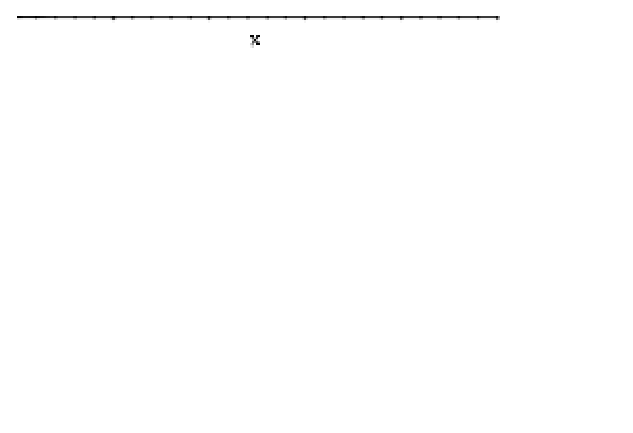
\includegraphics[
width=3in, \textwidth
]{HJC61301.jpg}
%\end{center}
%$$m\in\gz^{+}\;m\neq1$$%
%EndExpansion
\item Radical
es de la forma:$$y=ax^(1/n)$$
%TCIMACRO{\FRAME{dtbpFU}{3in}{2.0003in}{0pt}{\Qcb{$m\in\qz^{+}-\gz^{+}$}}%
%{}{Plot}{\special{ language "Scientific Word";  type "MAPLEPLOT";  width 3in;
%height 2.0003in;  depth 0pt;  display "PICT";  plot_snapshots TRUE;
%mustRecompute FALSE;  lastEngine "MuPAD";  xmin "-5";  xmax "5";
%xviewmin "0.001";  xviewmax "5.000000";  yviewmin "0.428825";
%yviewmax "2.272213";  viewset "XY";  plottype 4;  numpoints 49;
%plotstyle "patch";  axesstyle "normal";  xis \TEXUX{x};  yis \TEXUX{y};
%var1name \TEXUX{$x$};  var2name \TEXUX{$y$};  function \TEXUX{$\sqrt{x}$};
%linecolor "black";  linestyle 1;  pointstyle "point";  linethickness 1;
%lineAttributes "Solid";  var1range "-5,5";  num-x-gridlines 49;
%curveColor "[flat::RGB:0000000000]";  curveStyle "Line";  rangeset "X";
%valid_file "T";  tempfilename 'HJC6YV00.wmf';tempfile-properties "XPR";}}}%
%BeginExpansion
%\begin{center}
\centering
\includegraphics[
height=2.0003in,
width=3in
]{HJC6YV00.jpg)
%\end{center}
%$$m\in z^{+}- z^{+}$$%
%\item Inverso de la forma:
%\begin{equation}
%y=ax^(-n)
%\end{equqtion}
%\begin{center}
%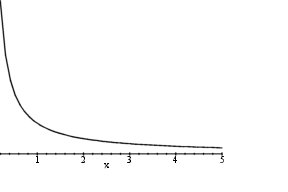
\includegraphics[
%height=2.0003in,
%width=3in
%]{HJC6YZ01.jpg}
%\end{center}
%%EndExpansion
%\item Directamente proporcional\\%
%es de la forma: $$y= ax^n$$
%\begin{center}
%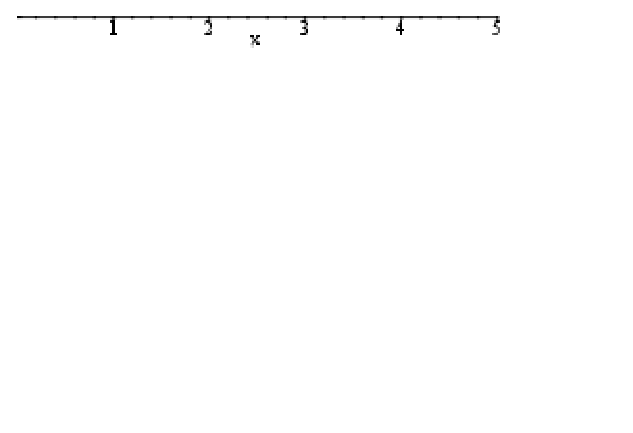
\includegraphics[
%height=2.0003in,
%width=3in
%]{HJC6Z202.jpg}%
%\end{center}
%%$$m=1\, y=mx$$
%%EndExpansion
%\item Se llama modelo exponencial a \\ $y=ae^{mx},\;\;a,m\in\rz,\;a,m\neq
%0$\newline%
%\begin{tabular}
%[c]{ll}%
%%TCIMACRO{\FRAME{itbpF}{4.6063cm}{5.0742cm}{0cm}{}{}{Plot}%
%%{\special{ language "Scientific Word";  type "MAPLEPLOT";  width 4.6063cm;
%%height 5.0742cm;  depth 0cm;  display "USEDEF";  plot_snapshots TRUE;
%%mustRecompute FALSE;  lastEngine "MuPAD";  xmin "-5";  xmax "5";
%%xviewmin "0.000012";  xviewmax "5.000000";  yviewmin "1.000";
%%yviewmax "3.440650";  viewset "XY";  plottype 4;  numpoints 49;
%%plotstyle "patch";  axesstyle "normal";  xis \TEXUX{x};  yis \TEXUX{y};
%%var1name \TEXUX{$x$};  var2name \TEXUX{$y$};  function \TEXUX{$e^{x}$};
%%linecolor "black";  linestyle 1;  pointstyle "point";  linethickness 1;
%%lineAttributes "Solid";  var1range "-5,5";  num-x-gridlines 49;
%%curveColor "[flat::RGB:0000000000]";  curveStyle "Line";  rangeset "X";
%%valid_file "T";  tempfilename 'HJC6Z303.wmf';tempfile-properties "XPR";}}}%
%%BeginExpansion
%\raisebox{-0cm}{\includegraphics[
%height=5.0742cm,
%width=4.6063cm
%]%
%{HJC6Z303.jpg}%
%}%
%%EndExpansion
%&
%%TCIMACRO{\FRAME{itbpF}{4.6063cm}{5.0742cm}{0cm}{}{}{Plot}%
%%{\special{ language "Scientific Word";  type "MAPLEPLOT";  width 4.6063cm;
%%height 5.0742cm;  depth 0cm;  display "USEDEF";  plot_snapshots TRUE;
%%mustRecompute FALSE;  lastEngine "MuPAD";  xmin "-5";  xmax "5";
%%xviewmin "0.000000";  xviewmax "5.000000";  yviewmin "0.004";
%%yviewmax "1.440650";  viewset "XY";  plottype 4;  numpoints 49;
%%plotstyle "patch";  axesstyle "normal";  xis \TEXUX{x};  yis \TEXUX{y};
%%var1name \TEXUX{$x$};  var2name \TEXUX{$y$};  function \TEXUX{$e^{-x}$};
%%linecolor "black";  linestyle 1;  pointstyle "point";  linethickness 1;
%%lineAttributes "Solid";  var1range "-5,5";  num-x-gridlines 49;
%%curveColor "[flat::RGB:0000000000]";  curveStyle "Line";  rangeset "X";
%%valid_file "T";  tempfilename 'HJC6Z404.wmf';tempfile-properties "XPR";}}}%
%%BeginExpansion
%\raisebox{-0cm}{\includegraphics[
%height=5.0742cm,
%width=4.6063cm
%]%
%{HJC6Z404.jpg}%
%}%
%%EndExpansion
%\end{tabular}
%\item Modelo logar\'{\i}tmico $y=\frac{1}{m}\ln x\;m\in\rz,\;m\neq0$%
%%TCIMACRO{\FRAME{dhF}{3in}{2.0003in}{0pt}{}{}{Plot}%
%%{\special{ language "Scientific Word";  type "MAPLEPLOT";  width 3in;
%%height 2.0003in;  depth 0pt;  display "USEDEF";  plot_snapshots TRUE;
%%mustRecompute FALSE;  lastEngine "MuPAD";  xmin "-5";  xmax "5";
%%xviewmin "1.000000";  xviewmax "5.000000";  yviewmin "0.001";
%%yviewmax "2.018052";  viewset "XY";  plottype 4;  numpoints 49;
%%plotstyle "patch";  axesstyle "normal";  xis \TEXUX{x};  yis \TEXUX{y};
%%var1name \TEXUX{$x$};  var2name \TEXUX{$y$};  function \TEXUX{$\log x$};
%%linecolor "black";  linestyle 1;  pointstyle "point";  linethickness 1;
%%lineAttributes "Solid";  var1range "-5,5";  num-x-gridlines 49;
%%curveColor "[flat::RGB:0000000000]";  curveStyle "Line";  rangeset "X";
%%valid_file "T";  tempfilename 'HJC6Z405.wmf';tempfile-properties "XPR";}}}%
%%BeginExpansion
%\begin{center}
%\includegraphics[
%height=2.0003in,
%width=3in
%]%
%{HJC6Z405.jpg}%
%\end{center}
%%EndExpansion
%\item Modelo lineal \\ $y=mx+b\;\;m,b\in\rz,\;m\neq0$%
%%TCIMACRO{\FRAME{dhF}{3in}{2.0003in}{0pt}{}{}{Plot}%
%%{\special{ language "Scientific Word";  type "MAPLEPLOT";  width 3in;
%%height 2.0003in;  depth 0pt;  display "USEDEF";  plot_snapshots TRUE;
%%mustRecompute FALSE;  lastEngine "MuPAD";  xmin "-5";  xmax "5";
%%xviewmin "-5.01";  xviewmax "5.01";  yviewmin "-2.01";  yviewmax "8.01";
%%plottype 4;  numpoints 49;  plotstyle "patch";  axesstyle "normal";
%%xis \TEXUX{x};  yis \TEXUX{y};  var1name \TEXUX{$x$};  var2name \TEXUX{$y$};
%%function \TEXUX{$x+3$};  linecolor "black";  linestyle 1;
%%pointstyle "point";  linethickness 1;  lineAttributes "Solid";
%%var1range "-5,5";  num-x-gridlines 49;  curveColor "[flat::RGB:0000000000]";
%%curveStyle "Line";  valid_file "T";
%%tempfilename 'HJC6Z706.wmf';tempfile-properties "XPR";}}}%
%%BeginExpansion
%\begin{center}
%\includegraphics[
%height=2.0003in,
%width=3in
%]%
%{HJC6Z706.jpg}%
%\end{center}
%%EndExpansion
%\item Modelo polinomico%
%%TCIMACRO{\FRAME{dtbpFUX}{3in}{2.0003in}{0pt}{\Qcb{$y=A_{n}x^{n}+A_{n-1}%
%%x^{n-1}+\cdots+A_{1}x+A_{0}$}}{}{Plot}{\special{ language "Scientific Word";
%%type "MAPLEPLOT";  width 3in;  height 2.0003in;  depth 0pt;
%%display "USEDEF";  plot_snapshots TRUE;  mustRecompute FALSE;
%%lastEngine "MuPAD";  xmin "-5";  xmax "5";  xviewmin "-5.01";
%%xviewmax "5.01";  yviewmin "-100.26";  yviewmax "160.26";  plottype 4;
%%numpoints 49;  plotstyle "patch";  axesstyle "normal";  xis \TEXUX{x};
%%yis \TEXUX{y};  var1name \TEXUX{$x$};  var2name \TEXUX{$y$};
%%function \TEXUX{$x^{3}+x^{2}+x+5$};  linecolor "black";  linestyle 1;
%%pointstyle "point";  linethickness 1;  lineAttributes "Solid";
%%var1range "-5,5";  num-x-gridlines 49;  curveColor "[flat::RGB:0000000000]";
%%curveStyle "Line";  valid_file "T";
%%tempfilename 'HJC75307.wmf';tempfile-properties "XPR";}}}%
%%BeginExpansion
%\begin{center}
%\fbox{\includegraphics[
%height=2.0003in,
%width=3in
%]%
%{HJC75307.jpg}%
%}
%\end{center}
%$$y=A_{n}x^{n}+A_{n-1}x^{n-1}+\cdots+A_{1}x+A_{0}$$%
%%EndExpansion
%\end{enumerate}
%\subsection{Ajuste de la curva}
%Al observar las gr\'{a}ficas notamos que muchas se parecen y a veces es
%d\'{\i}ficil estar seguro si el modelo que escogemos es adecuado, es m\'{a}s
%no conocemos todos los modelos. en esta secci\'{o}n explicaremos dos
%m\'{e}todos para ayudarnos a escoger un modelo que se aproxime de buena forma
%a los datos.
\end{descrsf}
\begin{descrsf}{linealizacion}
\item Linealizaci\'{o}n :\newline Este m\'{e}todo consiste en encontrar dos
relaciones $h\left(  y\right)  $ y $f\left(  x\right)  $ tales que al graficar
$h\left(  y\right)  $ vs $f\left(  x\right)  $ se obtenga una linea recta, es
decir si esto sucede el modelo es satisfactorio.\newline Por ejemplo si
tenemos los datos
\[%
\begin{tabular}
[c]{|l|l|l|l|l|l|}\hline
$y\left(  cm\right)  $ & 1 & 4 & 9 & 16 & 25\\\hline
$x(s)$ & 1 & 2 & 3 & 4 & 5\\\hline
\end{tabular}
\]
%TCIMACRO{\FRAME{dhF}{2.4111in}{1.8343in}{0pt}{}{}{potencial.wmf}%
%{\special{ language "Scientific Word";  type "GRAPHIC";
%maintain-aspect-ratio TRUE;  display "PICT";  valid_file "F";
%width 2.4111in;  height 1.8343in;  depth 0pt;  original-width 3.0415in;
%original-height 2.3056in;  cropleft "0";  croptop "1";  cropright "1";
%cropbottom "0";  filename 'D:/Tacho/potencial.WMF';file-properties "XNPEU";}%
%}}%
%BeginExpansion
%\begin{center}
\centering
\includegraphics[
height=1.8343in,
width=2.4111in
]%
{potencial.jpg}%
%\end{center}
%EndExpansion
De acuerdo con la forma el modelo es $y=ax^{m}$, pero si analizamos los datos
ellos nos hacen sospechar que $m=2,$ por lo que podr\'{\i}amos hacer $h\left(
y\right)  =y$ y $f\left(  x\right)  =x^{2}$ de lo que obtenemos la siguiente
tabla
\[%
\begin{tabular}
[c]{llllll}%
$h\left(  y\right)  $ & 1 & 4 & 9 & 16 & 25\\
$f\left(  x\right)  $ & 1 & 4 & 9 & 16 & 25
\end{tabular}
\]
%TCIMACRO{\FRAME{dhF}{3.3088in}{2.2762in}{0pt}{}{}{cuadra.wmf}%
%{\special{ language "Scientific Word";  type "GRAPHIC";
%maintain-aspect-ratio TRUE;  display "PICT";  valid_file "F";
%width 3.3088in;  height 2.2762in;  depth 0pt;  original-width 3.2638in;
%original-height 2.2364in;  cropleft "0";  croptop "1";  cropright "1";
%cropbottom "0";  filename 'D:/Tacho/cuadra.WMF';file-properties "XNPEU";}}}%
%BeginExpansion
%\begin{center}
\centering
\includegraphics[
height=2.2762in,
width=3.3088in
]%
{cuadra.jpg}%
%\end{center}
%EndExpansion
Como se obtuvo una recta podemos decir que el modelo es aceptable y al
determinar la ecuaci\'{o}n de la recta nos que al tomar dos puntos
cualesquiera
\[
a=\frac{y_{1}-y_{2}}{x_{1}^{2}-x_{2}^{2}}=\frac{16-9}{16-9}=1
\]
como la relaci\'{o}n matem\'{a}tica es $h\left(  y\right)  =af\left(
x\right)  , $ entonces queda $y=x^{2}.$\newline Este m\'{e}todo no es
pr\'{a}ctico en el sentido de que si no sospechamos nada acerca de la
relaci\'{o}matem\'{a}tica es casi imposible determinar $h\left(  y\right)  $ y
$f\left(  x\right)  ,$ afortunadamente para los modelos planteados ya existen
estas relaciones
\begin{descrsf}{modelos}
\item Para el modelo $y=ax^{m}$ son
\[
h\left(  y\right)  =\log y,\;f\left(  x\right)  =\log x
\]
al obtener la recta
%TCIMACRO{\FRAME{dtbpFU}{3.435in}{2.2485in}{0pt}{\Qcb{$\log Y=m\log
%x+b,a=10^{b}$}}{}{loglog.wmf}{\special{ language "Scientific Word";
%type "GRAPHIC";  maintain-aspect-ratio TRUE;  display "PICT";
%valid_file "F";  width 3.435in;  height 2.2485in;  depth 0pt;
%original-width 3.3892in;  original-height 2.2087in;  cropleft "0";
%croptop "1";  cropright "1";  cropbottom "0";
%filename 'D:/Tacho/loglog.WMF';file-properties "XNPEU";}}}%
%BeginExpansion
%\begin{center}
\centering
\includegraphics[
height=2.2485in,
width=3.435in
]%
{loglog.jpg}%
\\
$\log Y=m\log x+b,a=10^{b}$%
%\end{center}
%EndExpansion
podemos encontrar
\begin{align*}
m  & =\frac{\log y_{i}-\log y_{j}}{\log x_{i}-\log x_{j}}\\
a  & =\frac{y_{i}}{x_{i}^{m}}.
\end{align*}
En la pr\'{a}ctica debido a los errores al tomar diferentes parejas $\left(
x_{i},y_{i}\right)  $ los valores de $m$ y $a$ no son constantes, por lo que
hay que determinarlos varias veces y promediar los resultados, as\'{\i} la
relaci\'{o}n matem\'{a}tica queda $y=\bar{a}x^{\bar{m}}$
\item Para el modelo $y=ae^{mx}$ se escogen las relaciones
\[
h\left(  y\right)  =\ln y,\;f\left(  x\right)  =x
\]
y si obtenemos la recta
%TCIMACRO{\FRAME{dhFU}{3.435in}{2.2485in}{0pt}{\Qcb{$\ln Y=mX+b;\;a=e^{b}$}}%
%{}{semilog.wmf}{\special{ language "Scientific Word";  type "GRAPHIC";
%maintain-aspect-ratio TRUE;  display "PICT";  valid_file "F";  width 3.435in;
%height 2.2485in;  depth 0pt;  original-width 3.3892in;
%original-height 2.2087in;  cropleft "0";  croptop "1";  cropright "1";
%cropbottom "0";  filename 'D:/Tacho/semilog.WMF';file-properties "XNPEU";}}}%
%BeginExpansion
%\begin{center}
\centering
\includegraphics[
height=2.2485in,
width=3.435in
]%
{semilog.jpg}%
\\
$\ln Y=mX+b;\;a=e^{b}$%
%\end{center}
%EndExpansion
podemos utilizar
\begin{align*}
m  & =\frac{\ln y_{i}-\ln y_{j}}{x_{i}-x_{j}}\\
a  & =\frac{y_{i}}{e^{mx_{i}}}.
\end{align*}
y calculamos varios valores de $m$ y $a$ para promediarlos y obtener la
relaci\'{o}n matem\'{a}tica $y=\bar{a}e^{\bar{m}x}$
\item Si el modelo es $y=\frac{1}{m}\ln x$ las relaciones son
\[
h\left(  y\right)  =y,\;f\left(  x\right)  =\ln x
\]
si la gr\'{a}fica $f\left(  x\right)  \;vs\;h\left(  y\right)  $ es lineal
como se muestra en la figura
%TCIMACRO{\FRAME{dhF}{2.6593in}{1.8334in}{0pt}{}{}{logm.wmf}%
%{\special{ language "Scientific Word";  type "GRAPHIC";
%maintain-aspect-ratio TRUE;  display "PICT";  valid_file "F";
%width 2.6593in;  height 1.8334in;  depth 0pt;  original-width 6.1531in;
%original-height 4.222in;  cropleft "0";  croptop "1";  cropright "1";
%cropbottom "0";  filename 'D:/Tacho/logm.WMF';file-properties "XNPEU";}}}%
%BeginExpansion
%\begin{center}
\centering
\includegraphics[
height=1.8334in,
width=2.6593in
]%
{logm.jpg}%
%\end{center}
%EndExpansion
podemos usar
\[
m=\frac{\ln x_{i}-\ln x_{j}}{y_{i}-y_{j}}%
\]
calculamos $m$ varias veces y obtenemos $y=\frac{1}{\bar{m}}\ln x.$
\item El modelo lineal es trivial por lo que dejamos de tarea al lector
\end{descrsf}{Data Studio}
\item Usando Data Studio es f\'{a}cil realizar el ajuste \newline Se seleciona
la regi\'{o}n de la curva que nos intersa y lugego escogemos en la barra de
herramienta fit y se escoge el modelo adecuado de acuerdcon los siguientes
par\'{a}metros:%
%TCIMACRO{\FRAME{fhF}{0.6356in}{1.0326in}{0pt}{}{}{ajuste.jpg}%
%{\special{ language "Scientific Word";  type "GRAPHIC";
%maintain-aspect-ratio TRUE;  display "USEDEF";  valid_file "F";
%width 0.6356in;  height 1.0326in;  depth 0pt;  original-width 0.6045in;
%original-height 0.9997in;  cropleft "0";  croptop "1";  cropright "1";
%cropbottom "0";  filename 'ajuste.jpg';file-properties "XNPEU";}}}%
%BeginExpansion
%\begin{figure}
%[h]
%\begin{center}
\centering
\includegraphics[
height=1.0326in,
width=0.6356in
]%
{ajuste.jpg}%
%\end{center}
%end{figure}
%EndExpansion
\begin{descrsf}{ajuste}
\item Si se escoge el modelo lineal obtenemos un display parecido al de la
figura%
%TCIMACRO{\FRAME{dhF}{1.8922in}{1.0326in}{0pt}{}{}{ajuste1.jpg}%
%{\special{ language "Scientific Word";  type "GRAPHIC";
%maintain-aspect-ratio TRUE;  display "USEDEF";  valid_file "F";
%width 1.8922in;  height 1.0326in;  depth 0pt;  original-width 1.8542in;
%original-height 0.9997in;  cropleft "0";  croptop "1";  cropright "1";
%cropbottom "0";  filename 'ajuste1.jpg';file-properties "XNPEU";}}}%
%BeginExpansion
%\begin{center}
\centering
\includegraphics[
height=1.0326in,
width=1.8922in
]%
{ajuste1.jpg}%
%\end{center}
%EndExpansion
y se dice que el modelo es bueno si $r^{2}>0.95$
\item Si se escoge otro modelo obtendremos un display como%
%TCIMACRO{\FRAME{dbhF}{2.0807in}{1.2107in}{0pt}{}{}{ajuste2.jpg}%
%{\special{ language "Scientific Word";  type "GRAPHIC";
%maintain-aspect-ratio TRUE;  display "USEDEF";  valid_file "F";
%width 2.0807in;  height 1.2107in;  depth 0pt;  original-width 2.0418in;
%original-height 1.177in;  cropleft "0";  croptop "1";  cropright "1";
%cropbottom "0";  filename 'ajuste2.jpg';file-properties "XNPEU";}}}%
%BeginExpansion
%\begin{center}
\centering
\includegraphics[
height=1.2107in,
width=2.0807in
]%
{ajuste2.jpg}%
%\end{center}
%EndExpansion
y decimos que el modelo es bueno si el mean Square Error es despreciable
comparado con $\bar{y}$
\item Ajuste lineal\newline El ajuste lineal es un m\'{e}todo
estad\'{\i}stico, parecido al anterior, pero usando herramientas
diferentes.\newline En este caso no explicaremos mucho , s\'{o}lo plantearemos
algunas f\'{o}rmulas e interpretaremos los resultados \newline Si tenemos dos
conjuntos de datos
\begin{align*}
& x_{1},x_{2},x_{3},\cdots,x_{n}\\
& y_{1},y_{2},y_{3},\cdots,y_{n}%
\end{align*}
\end{descrsf}
definiremos la
\begin{descrsf}{an�lisis}
\item Media aritm\'{e}tica
\begin{align*}
\bar{x}  & =\frac{\sum_{i=1}^{n}x_{i}}{n}\\
\bar{y}  & =\frac{\sum_{i=1}^{n}y_{i}}{n}%
\end{align*}
\item Varianza
\begin{align*}
S_{xx}^{2}  & =\frac{\sum_{i=1}^{n}(x_{i}-\bar{x})^{2}}{n-1}\\
S_{yy}^{2}  & =\frac{\sum_{i=1}^{n}(y_{i}-\bar{y})^{2}}{n-1}%
\end{align*}
\item Covarianza
\[
S_{xy}=\frac{\sum_{i=1}^{n}(x_{i}-\bar{x})(y_{i}-\bar{y})}{n-1}%
\]
\item Coeficiente de correlaci\'{o}n
\[
r=\frac{S_{xy}}{\sqrt{S_{xx}^{2}S_{yy}^{2}}}%
\]
Cuando estudiamos dos variables $X\;$y $Y$, en realidad estas variables estas
variables tienen desde el punto de vista geom\'{e}trico el comportamiento de
dos vectores (rayos con direcci\'{o}n). Y se dice que existe un ajuste lineal
si los vectores representados por las desviaciones est\'{a}n alineados o son
paralelos.\newline Para determinar si esto sucede podemos utilizar la
trigonometr\'{\i}a para determinar el \'{a}ngulo entre los vectores
representados en la figura
%TCIMACRO{\FRAME{dhF}{1.8152in}{1.4659in}{0pt}{}{}{veca.wmf}%
%{\special{ language "Scientific Word";  type "GRAPHIC";
%maintain-aspect-ratio TRUE;  display "PICT";  valid_file "F";
%width 1.8152in;  height 1.4659in;  depth 0pt;  original-width 1.7781in;
%original-height 1.4304in;  cropleft "0";  croptop "1";  cropright "1";
%cropbottom "0";  filename 'D:/Tacho/veca.WMF';file-properties "XNPEU";}}}%
%BeginExpansion
%\begin{center}
\centering
\includegraphics[
height=1.4659in,
width=1.8152in
]%
{veca.jpg}%
%\end{center}
%EndExpansion
\end{descrsf}
\end{descrsf}
Utilizando una rama de las matem\'{a}ticas llamada algebra lineal se puede
comprobar que si $\theta$ es el \'{a}ngulo entre los vectores entonces
\[
\cos\theta=r
\]
Es decir este coeficiente determina la relaci\'{o}n lineal entre las
desviaciones de las variables y esta dependencia es perfecta cuando $r=\pm1$
existe el ajuste lineal en la practica esto no sucede debido a los errores
pero decimos que el ajuste es aceptable si $r^{2}>0.95.\;$\newline Si el
ajuste existe deben existir dos relaciones $h\left(  y\right)  $ y $f\left(
x\right)  $ tal que el modelo
\[
h\left(  y\right)  =mf\left(  x\right)  +b
\]
debe tener un $r$ adecuado \ y se puede calcular
\[
r=\frac{n\sum_{i.j=1}^{n}f\left(  x_{i}\right)  h\left(  y_{j}\right)
-\sum_{i=1}^{n}f\left(  x_{i}\right)  \sum_{j=1}^{n}h\left(  y_{i}\right)
}{\sqrt{\left[  n\sum_{i=1}^{n}f^{2}\left(  x_{i}\right)  -\left(  \sum
_{i=1}^{2}f\left(  x_{i}\right)  ^{2}\right)  \right]  }\left[  n\sum
_{j=1}^{n}h^{2}\left(  y_{j}\right)  -\left(  \sum_{j=1}^{2}h\left(
y_{j}\right)  ^{2}\right)  \right]  }%
\]
%
\begin{align*}
m  & =\frac{n\sum_{i.j=1}^{n}f\left(  x_{i}\right)  h\left(  y_{j}\right)
-\sum_{i=1}^{n}f\left(  x_{i}\right)  \sum_{j=1}^{n}h\left(  y_{i}\right)
}{n\sum_{i=1}^{n}f^{2}\left(  x_{i}\right)  -\left(  \sum_{i=1}^{2}f\left(
x_{i}\right)  ^{2}\right)  }\\
b  & =\frac{\sum_{j=1}^{n}h\left(  y_{j}\right)  -m\sum_{i=1}^{n}f\left(
x_{i}\right)  }{n}%
\end{align*}
donde \ $a$ se obtiene
\begin{itemize}
\item $a=10^{b}$ en el modelo $y=ax^{m}$
\item $a=e^{b}$ en el modelo $y=ae^{mx}$
\end{itemize}
\subsection{Interpretaci\'{o}n geom\'{e}trica de la covarianza}
Si consideramos una nube de puntos formados por las parejas de los datos
concretos de dos variables $X$ e $Y$ $\left(  x_{i},y_{i}\right)  $ el centro
de gravedad de esta nube de puntos es $\left(  \overset{-}{x},\overset{-}%
{y}\right)  $, ahora si trasladamos los ejes de tal forma que este punto sea
el centro, la nube queda dividida en cuatro cuadrantes los que indica que los
puntos que se encuentran en el pimer y tercer cuadrate contribuyen
positivamente al valor de la covarianza y los que se encuentran en los otros
dos cuadrantes contribuyen negativamente. como lo indica la figura.a y si los
puntos se reparten con igual proporci\'{o}n la covarianza ser\'{a} negativa
como indica la segunda gr\'{a}fica de la figura a%
%TCIMACRO{\FRAME{ftbpFU}{3.0528in}{1.817in}{0pt}{\Qcb{fig a}}{}{fig4.wmf}%
%{\special{ language "Scientific Word";  type "GRAPHIC";
%maintain-aspect-ratio TRUE;  display "USEDEF";  valid_file "F";
%width 3.0528in;  height 1.817in;  depth 0pt;  original-width 5.6351in;
%original-height 3.333in;  cropleft "0";  croptop "1";  cropright "1";
%cropbottom "0";  filename 'D:/Tacho/fig4.wmf';file-properties "XNPEU";}}}%
%BeginExpansion
%\begin{figure}
%[ptb]
%\begin{center}
\centering
\includegraphics[
height=1.817in,
width=3.0528in
]%
{fig4.jpg}%
\caption{fig a}%
%\end{center}
%\end{figure}
%EndExpansion
y no hay relaci\'{o}n matem\'{a}tica si la nube de puntos no tiene ninguna
tendencia como en la fig b%
%TCIMACRO{\FRAME{dhFU}{2.7743in}{1.817in}{0pt}{\Qcb{fig b}}{}{fig4cb.wmf}%
%{\special{ language "Scientific Word";  type "GRAPHIC";
%maintain-aspect-ratio TRUE;  display "USEDEF";  valid_file "F";
%width 2.7743in;  height 1.817in;  depth 0pt;  original-width 5.6455in;
%original-height 3.6772in;  cropleft "0";  croptop "1";  cropright "1";
%cropbottom "0";  filename 'D:/Tacho/fig4cb.wmf';file-properties "XNPEU";}}}%
%BeginExpansion
%\begin{center}
\centering
\includegraphics[
height=1.817in,
width=2.7743in
]%
{fig4cb.jpg}%
\\
fig b
%\end{center}
%EndExpansion
\end{slide}
\end{document}
